\subsection{Spectral Risk Measures}\label{subsec:spectral-risk-measures}
Tthe spectral risk measures (SRM) of a hedged portfolio return $R^h$ has a form

\begin{align}
	\rho_\phi(R^h) = - \int_0^1 \phi(p) F_{R^h}^{(-1)}(p)\dd p,
	\end{align}

where $p$ is the loss quantile and $\phi(p)$ is a user-defined weighting function defined over $[0,1]$. \medskip

\natp{\em [Add properties on $\phi$! (Nonnegative, etc.)]}

Spectral risk measures can also be written as
\begin{align}
	\rho_\phi(R^h) = - \int_\mathbb{R} x f_{R^h}(x) \phi\{F_{R^h}(x)\} \dd x.
	\end{align}

Value-at-Risk (VaR) and Expected Shortfall (ES) fall in to the class of SRM.
VaR at the $\alpha$-confidence level is

\begin{align}
	\text{VaR}_\alpha = - F_{R^h}^{(-1)}(1-\alpha)
	\end{align};
ES at the $\alpha$-confidence level is \natp{\em [Please check, there
  should be a minus in front of the ES expression, just as with VaR.]}
\begin{align}
	\text{ES}_\alpha = -\frac{1}{1-\alpha}\int_{-\infty}^{\alpha} F_{R^h}^{(-1)}(p) \dd p
	\end{align}.
The VaR's $\phi(p)$ gives all its weight on the $\alpha$ quantile of $R^h$ and zero elsewhere, i.e. the weighting function is a Dirac delta function.
The ES' $\phi(p)$ gives all tail quantiles the same weight of $\frac{1}{1-\alpha}$ and non-tail quantiles zero weight. \medskip

Spectral risk measures take account of investor's risk aversion by using different $\phi(p)$.
Exponential spectral risk measures (ERM) as a kind of spectral risk measure take a form of the weight function

\begin{align}
	\phi(p) =\frac{k e^{-k(1-p)}}{1-e^{-k}} ,
	\end{align}
where $k$ is the Arrow-Pratt coefficient of absolute risk aversion. \medskip

$k$ has an economic interpretation of being the ratio between the second derivative and first derivative
of investor's utility function on an risky asset

\begin{align}
	k = -\frac{U''(x)}{U'(x)},
	\end{align}
for $x$ in all possible outcomes.
A summary of risk measures being used in portfolio selection probelm can be found in \citet{hardle2008applied}.\medskip

In this hedging study, variance and the risk measures mentioned above serve as a loss function determining the optimality
of $h^\ast$.

\begin{figure}[h]
	\begin{center}
		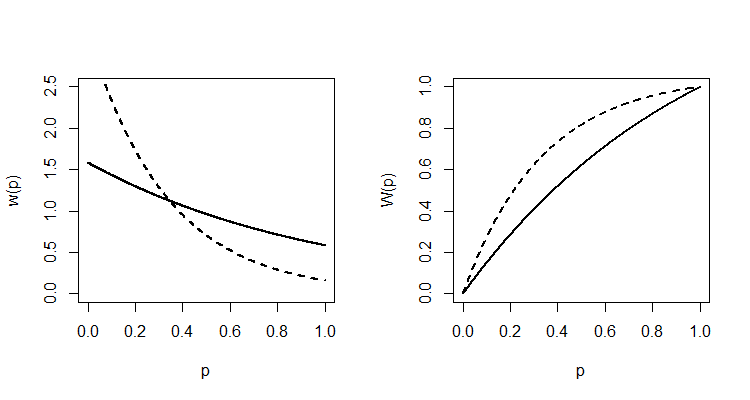
\includegraphics[scale = 0.7]{Figures/Fig1-1.png}\\
		%\vspace*{-10pt}\quantnet \href{https://github.com/mangrou/SRM/blob/master/SRM_QF/SRM_QF.m}{SRM\_QF}
	\end{center}
	\caption{Exponential SRMs for $k=1$ (dashed) and $k=2$ (solid).}\label{Fig1:EPSRM}
\end{figure}
